\section{Combined Model} \label{sec:CombinedModel}
The model derived is presented as the equations that constitute it and a block diagram. The simulations carried out are also depicted and compared.
\subsection{Attitude Model Equations}
\begin{itemize}
	\item Non-linear equations
	\begin{align}
		J_x\cdot\ddot{\phi}&=k_{th} \cdot(\omega^2_4-\omega^2_2) \cdot L &\\
		J_y \cdot\ddot{\theta}&=k_{th} \cdot(\omega^2_1-\omega^2_3) \cdot L &\\
		J_z\cdot\ddot{\psi}&=k_d \cdot(\omega^2_1-\omega^2_2+\omega^2_3-\omega^2_4)
		\label{eq:AngleEqVelocitiescombined}
	\end{align}
	\item Linearized equations
	\begin{flalign}
		J_x\cdot\Delta\ddot{\phi}   &= 2 \cdot k_{th} \cdot L \cdot({\overline{\omega}_4}\cdot \Delta \omega_2-{\overline{\omega}_2}\cdot \Delta \omega_4) \\
		J_y\cdot\Delta\ddot{\theta} &= 2 \cdot k_{th} \cdot L \cdot({\overline{\omega}_1}\cdot \Delta \omega_1-{\overline{\omega}_3}\cdot \Delta \omega_3) \\
		J_z\cdot\Delta\ddot{\psi}   &= 2 \cdot k_d \cdot ({\overline{\omega}_1}\cdot \Delta \omega_1-{\overline{\omega}_2}\cdot \Delta \omega_2+{\overline{\omega}_3}\cdot \Delta \omega_3-{\overline{\omega}_4}\cdot \Delta \omega_4)
	\end{flalign} \label{eqAngleLincombined}
\end{itemize}

\subsection{Translational Model Equations}
\begin{itemize}
	\item Non-linear equations
	\begin{flalign}
		\eq{m\cdot\ddot{x}_I}{-k_{th}\cdot({\omega_1}^2+{\omega_2}^2+{\omega_3}^2+{\omega_4}^2)\cdot\sin(\theta)} &\\
		\eq{m\cdot\ddot{y}_I}{-k_{th}\cdot({\omega_1}^2+{\omega_2}^2+{\omega_3}^2+{\omega_4}^2)\cdot(-\sin(\phi))\cdot\cos(\theta)} &\\
		\eq{m\cdot\ddot{z}_I}{F_g-k_{th}\cdot({\omega_1}^2+{\omega_2}^2+{\omega_3}^2+{\omega_4}^2)\cdot\cos(\phi)\cdot\cos(\theta)}
		\label{eq:AccelerationEqInertialVelocitiescombined}
	\end{flalign}
	\item Linearized equations 
	\begin{flalign}
		m\cdot\Delta\ddot{x}_I &= -k_{th}\cdot({\overline{\omega}_1}^2+{\overline{\omega}_2}^2+{\overline{\omega}_3}^2+{\overline{\omega}_4}^2)\cdot\cos(\overline{\theta})\Delta\theta &\\
		m\cdot\Delta\ddot{y}_I &=  k_{th}\cdot({\overline{\omega}_1}^2+{\overline{\omega}_2}^2+{\overline{\omega}_3}^2+{\overline{\omega}_4}^2)\cdot\cos(\overline{\phi})\cdot\cos(\overline{\theta})\cdot\Delta\phi &\\
		m\cdot\Delta\ddot{z}_I &= -2\textbf{ }k_{th}\cdot({\overline{\omega}_1}\cdot\Delta\omega_1+{\overline{\omega}_2}\cdot\Delta\omega_2+{\overline{\omega}_3}\cdot\Delta\omega_3+{\overline{\omega}_4}\cdot\Delta\omega_4)\cdot\cos(\overline{\phi})\cdot\cos(\overline{\theta})
	\end{flalign} \label{eq:FinalLinearEquationscombined}
\end{itemize}

\subsection{Linearized Block Diagrams}
\begin{figure}[H]
	\centering
	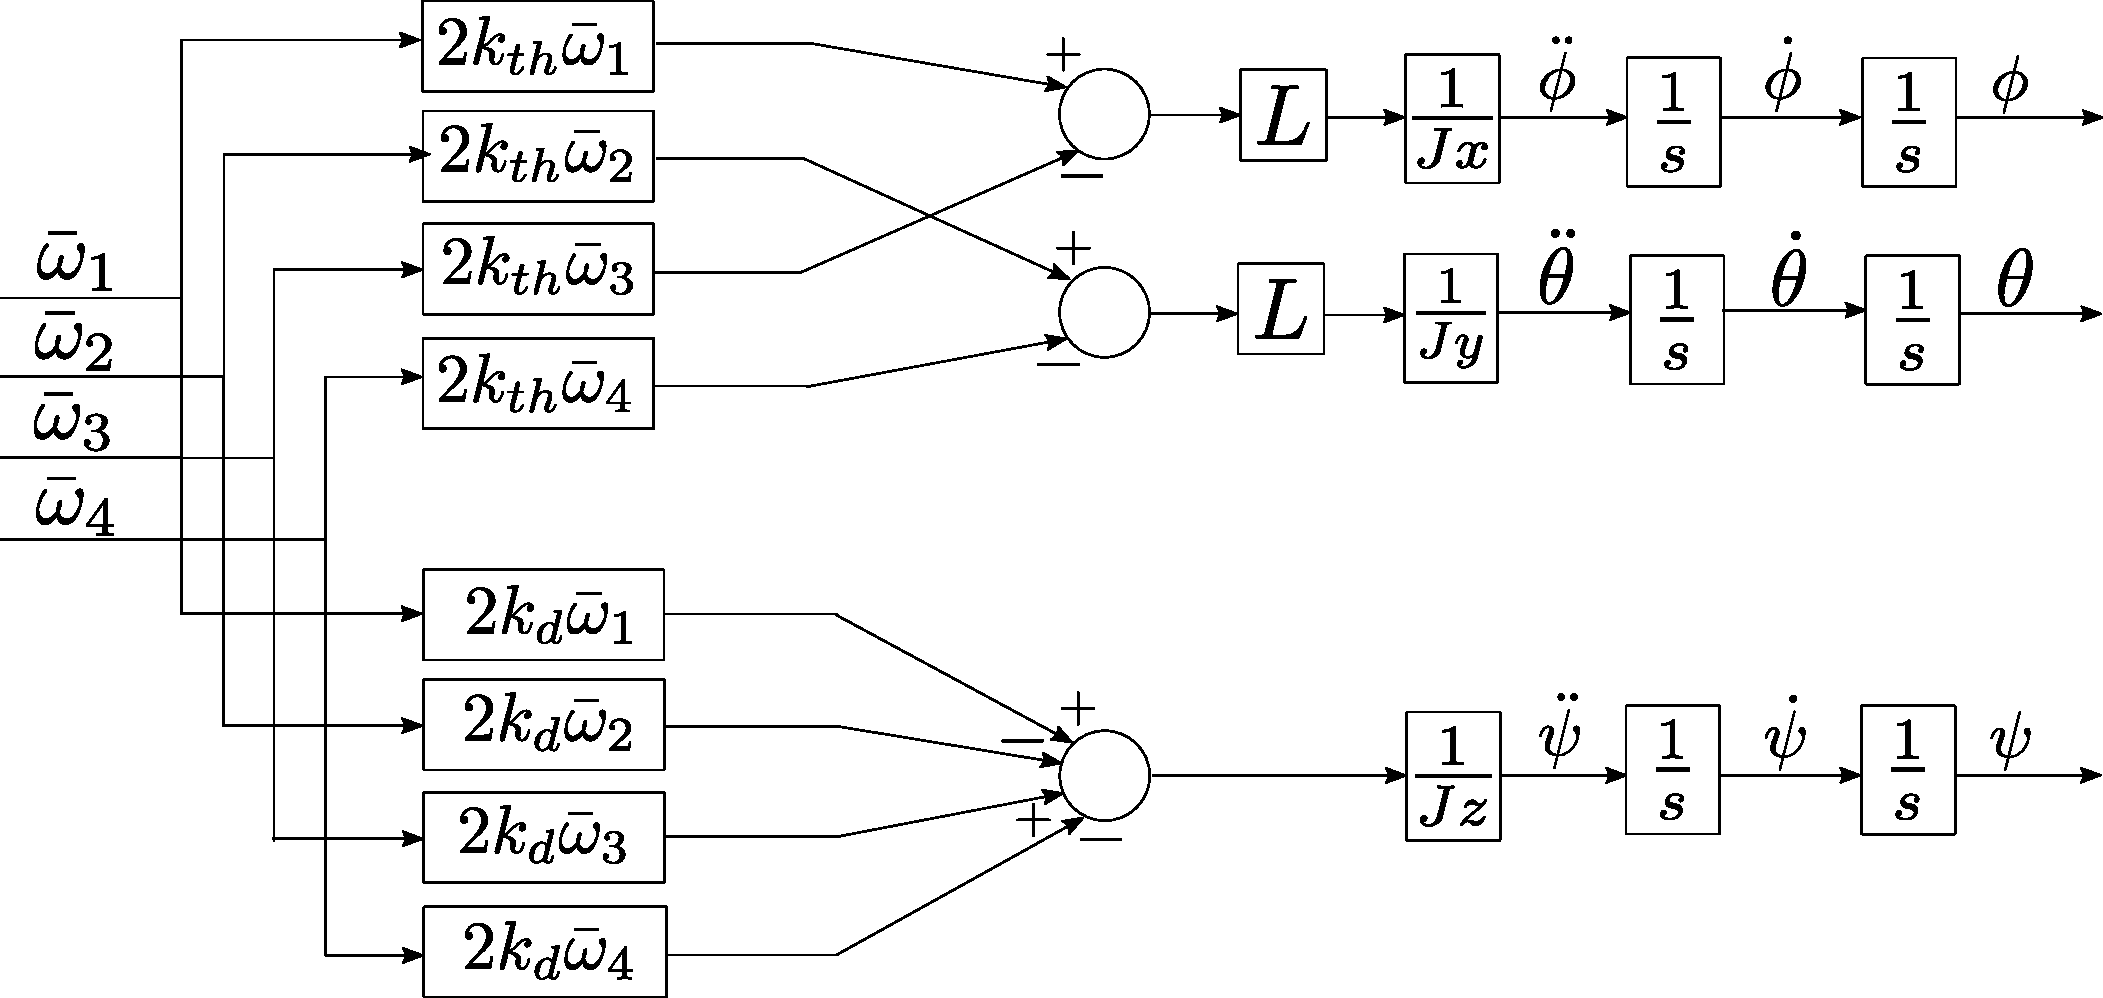
\includegraphics[scale=0.45]{figures/LinearModelBlockDiagram.pdf}
	\caption{.}
	\label{fig:LinearModelBlockDiagram}
\end{figure}

\subsection{Simulation}
The simulation of the model is done in Simulink. The parameters used for the simulations are shown in \autoref{ParametersQuadcopter}.
\begin{table}[H]
	\centering
	\begin{tabular}{|l|l|l|p{3cm}|}
		\hline %-----------------------------------------------------------------------------------
		\textbf{Parameter Name}&\textbf{Symbol} &\textbf{Value} &\textbf{Units}\\
		\hline %-----------------------------------------------------------------------------------
		Mass of the quadcopter  & $m$ & 0.996       &kg\\
		\hline
		%-----------------------------------------------------------------------------------
		Moment of inertia around x axis       & $J_x$  & 0.01073       & $kg \cdot m^2$\\
		\hline %-----------------------------------------------------------------------------------
		Moment of inertia around y axis       & $J_y$  & 0.01073       & $kg \cdot m^2$\\
		\hline %-----------------------------------------------------------------------------------
		Moment of inertia around z axis       & $J_z$  & 0.02135       & $kg \cdot m^2$\\
		\hline %-----------------------------------------------------------------------------------
		Length of quadcopter rm       & $L$  &   0.225       & $m$\\
		\hline %-----------------------------------------------------------------------------------
		Thrust force constant       & $k_{th}$  & -       & $kg \cdot m^2$\\
		\hline %-----------------------------------------------------------------------------------\\
		Drag torque constant      & $k_{d}$  & -       & $kg \cdot m^2$\\
		\hline %-----------------------------------------------------------------------------------\\
	\end{tabular}
	\caption{Parameters used in the simulation of the model.}
	\label{ParametersQuadcopter}
\end{table}\vspace{-18pt}

\begin{figure}[H]
	\centering
	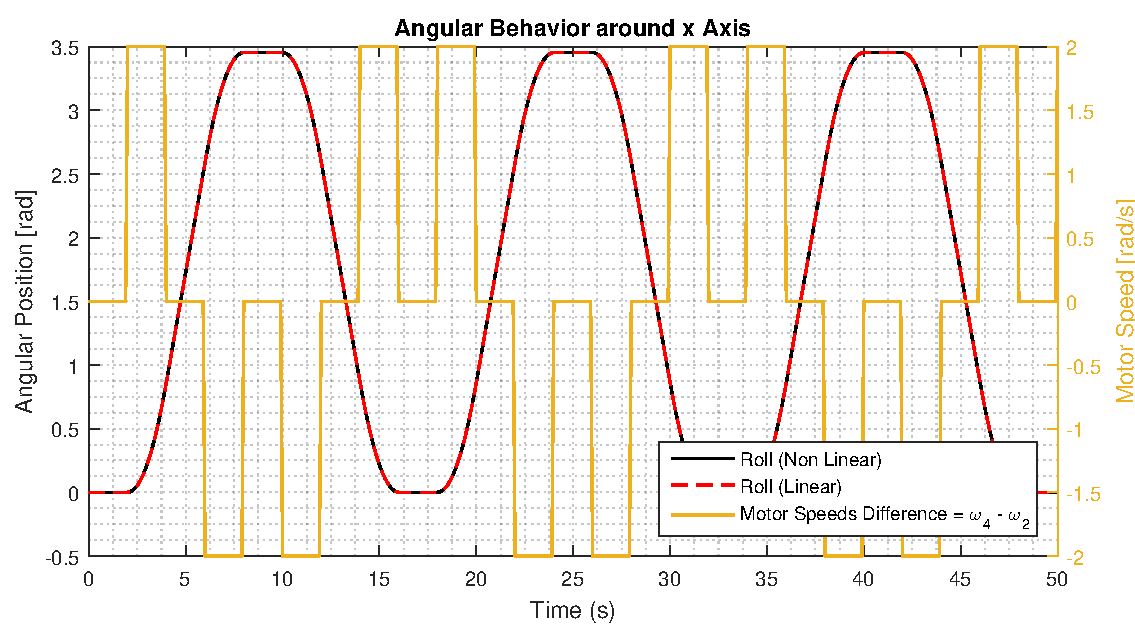
\includegraphics[scale=0.65]{figures/rollCompModel}
	\caption{.}
	\label{fig:rollCompModel}
\end{figure}

\begin{figure}[H]
	\centering
	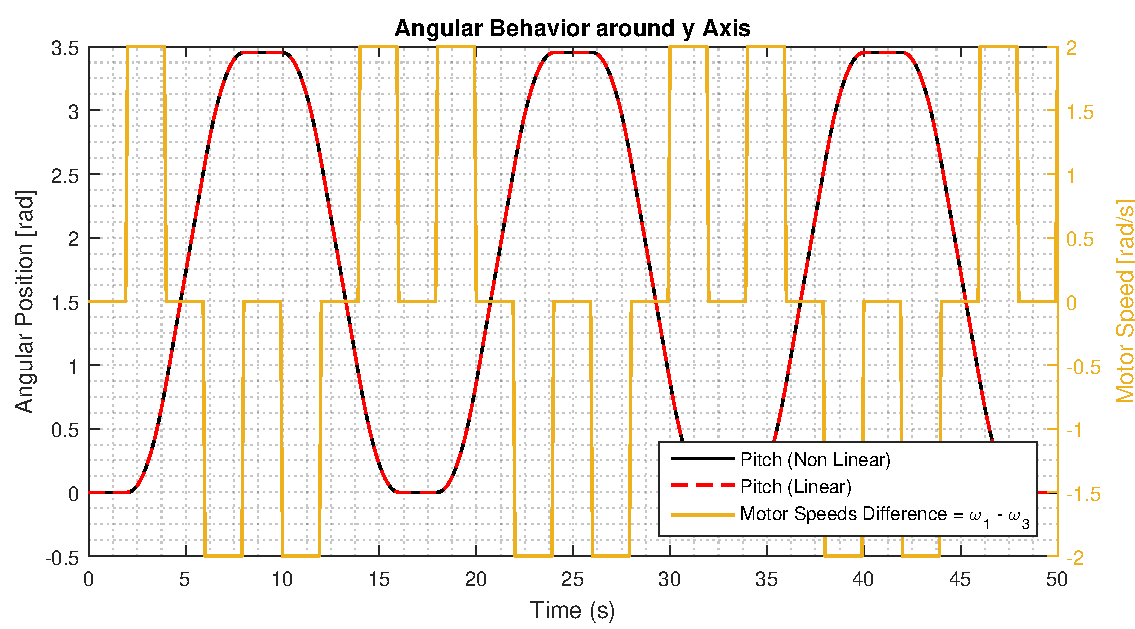
\includegraphics[scale=0.65]{figures/pitchCompModel}
	\caption{.}
	\label{fig:pitchCompModel}
\end{figure}

\begin{figure}[H]
	\centering
	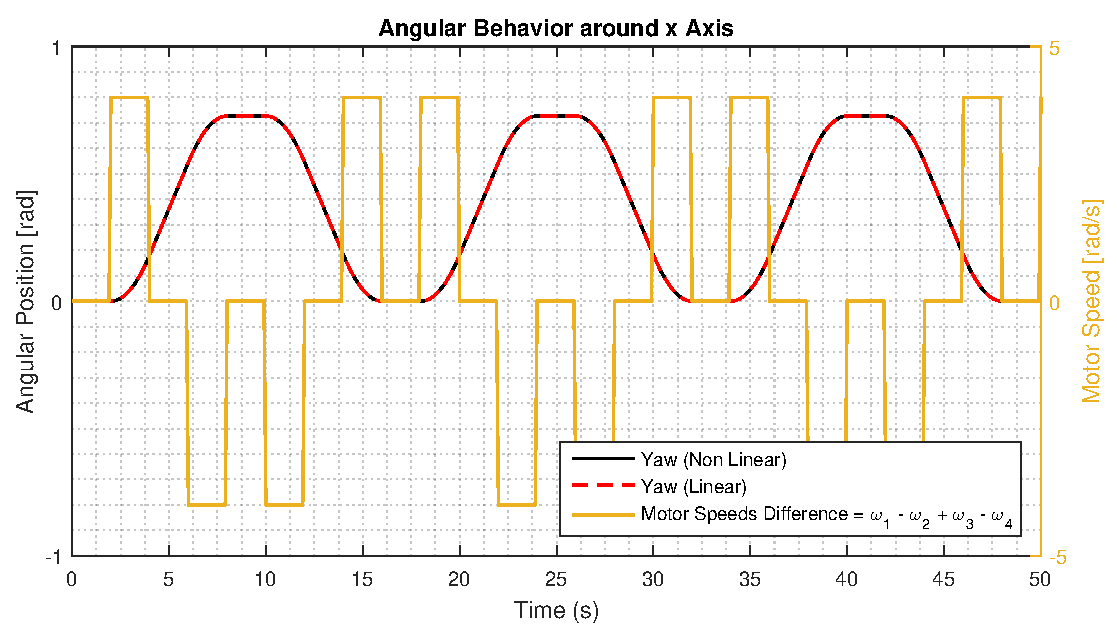
\includegraphics[scale=0.55]{figures/yawCompModel}
	\caption{.}
	\label{fig:yawCompModel}
\end{figure}
\fxnote{Title should say z-axis}

\begin{figure}[H]
	\centering
	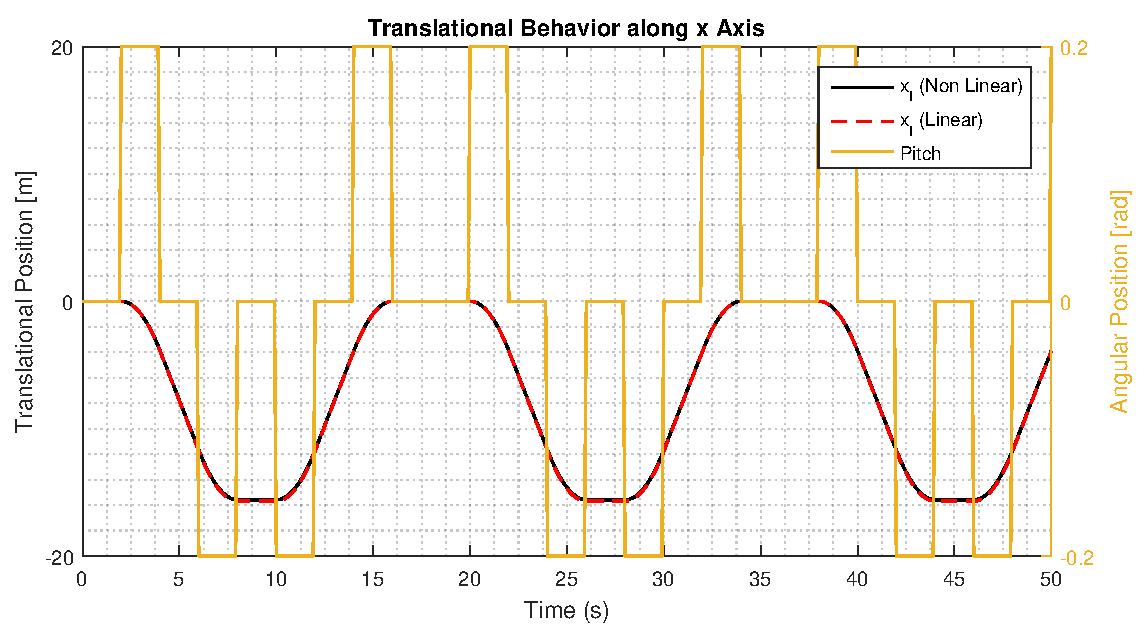
\includegraphics[scale=0.55]{figures/xCompModel}
	\caption{.}
	\label{fig:xCompModel}
\end{figure}

\begin{figure}[H]
	\centering
	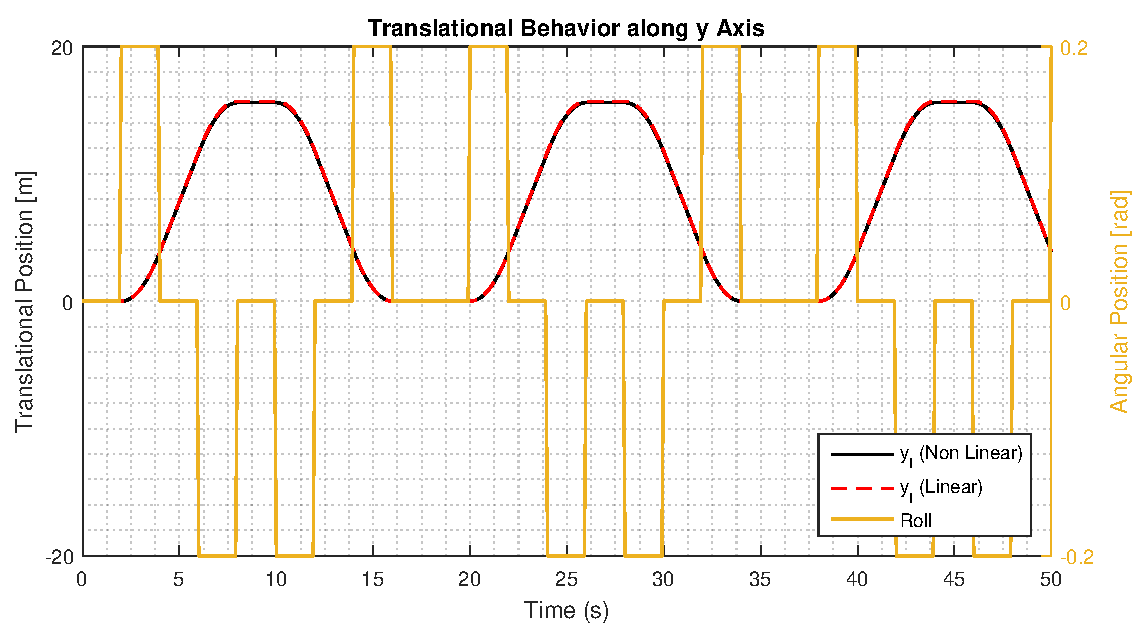
\includegraphics[scale=0.55]{figures/yCompModel}
	\caption{.}
	\label{fig:yCompModel}
\end{figure}

\begin{figure}[H]
	\centering
	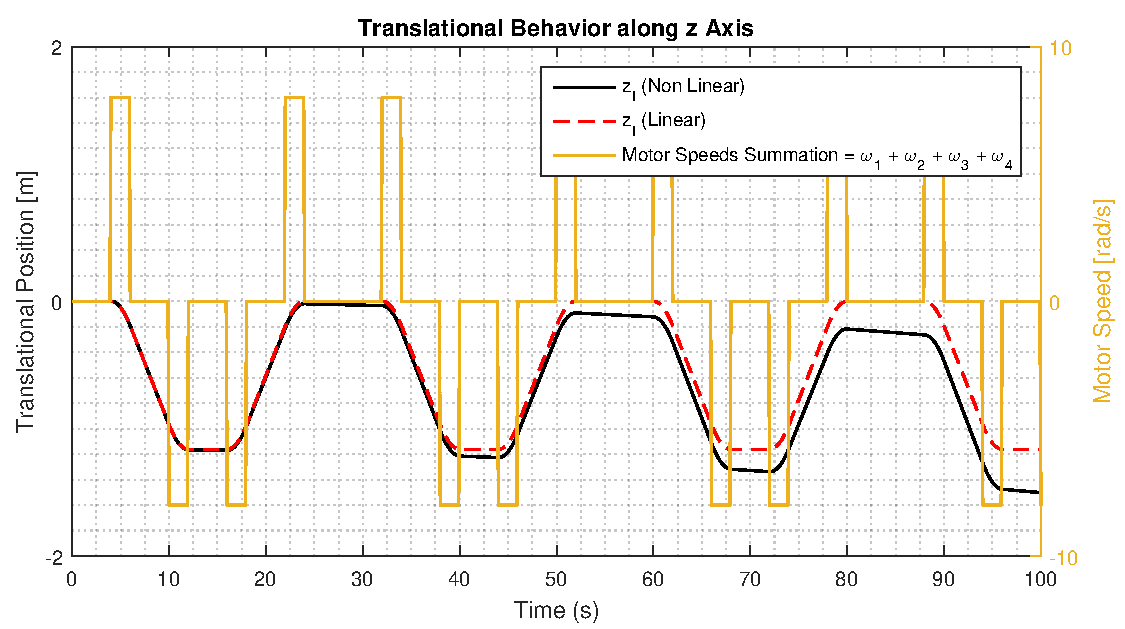
\includegraphics[scale=0.55]{figures/zCompModel}
	\caption{.}
	\label{fig:zCompModel}
\end{figure}
